\bibliography{dissertation}
\appendix

\chapter{AI Usage}
\label{appx:ai_prompt}

I did not directly prompt any Large Language Models, or any other AI model, to assist with the writing of my dissertation or implementation. However, as listed in the Supporting Technologies list, I used GitHub Copilot to help with writing some tests for the parser and type checker. I used it via the VS Code extension, which uses the context of your file, to provide advanced AI autocompletion.

% =============================================================================

\chapter{Tokens for Lexical Analysis}
\label{appx:tokens}
Below is the code for how tokens outputted by lexical analysis are defined. 
\begin{lstlisting}
enum TokenType {
    EOF,
    Newline,

    Id,
    UppercaseId,

    If,
    Then,
    Else,

    Match,
    LBrace,
    RBrace,

    IntLit,
    FloatLit,
    StringLit,
    CharLit,
    BoolLit,

    DoubleColon,
    RArrow,
    Forall,
    KWType,
    KWData,

    LParen,
    RParen,

    Lambda,

    Dollar,
    Dot,
    Comma,
    Bar,

    Assignment,
}

struct Token {
    tt: TokenType,
    value: String,
}
\end{lstlisting}

\chapter{How the System Looked During Various Testing Stages}
\section{Testathon}

\begin{figure}[h]
    \centering
    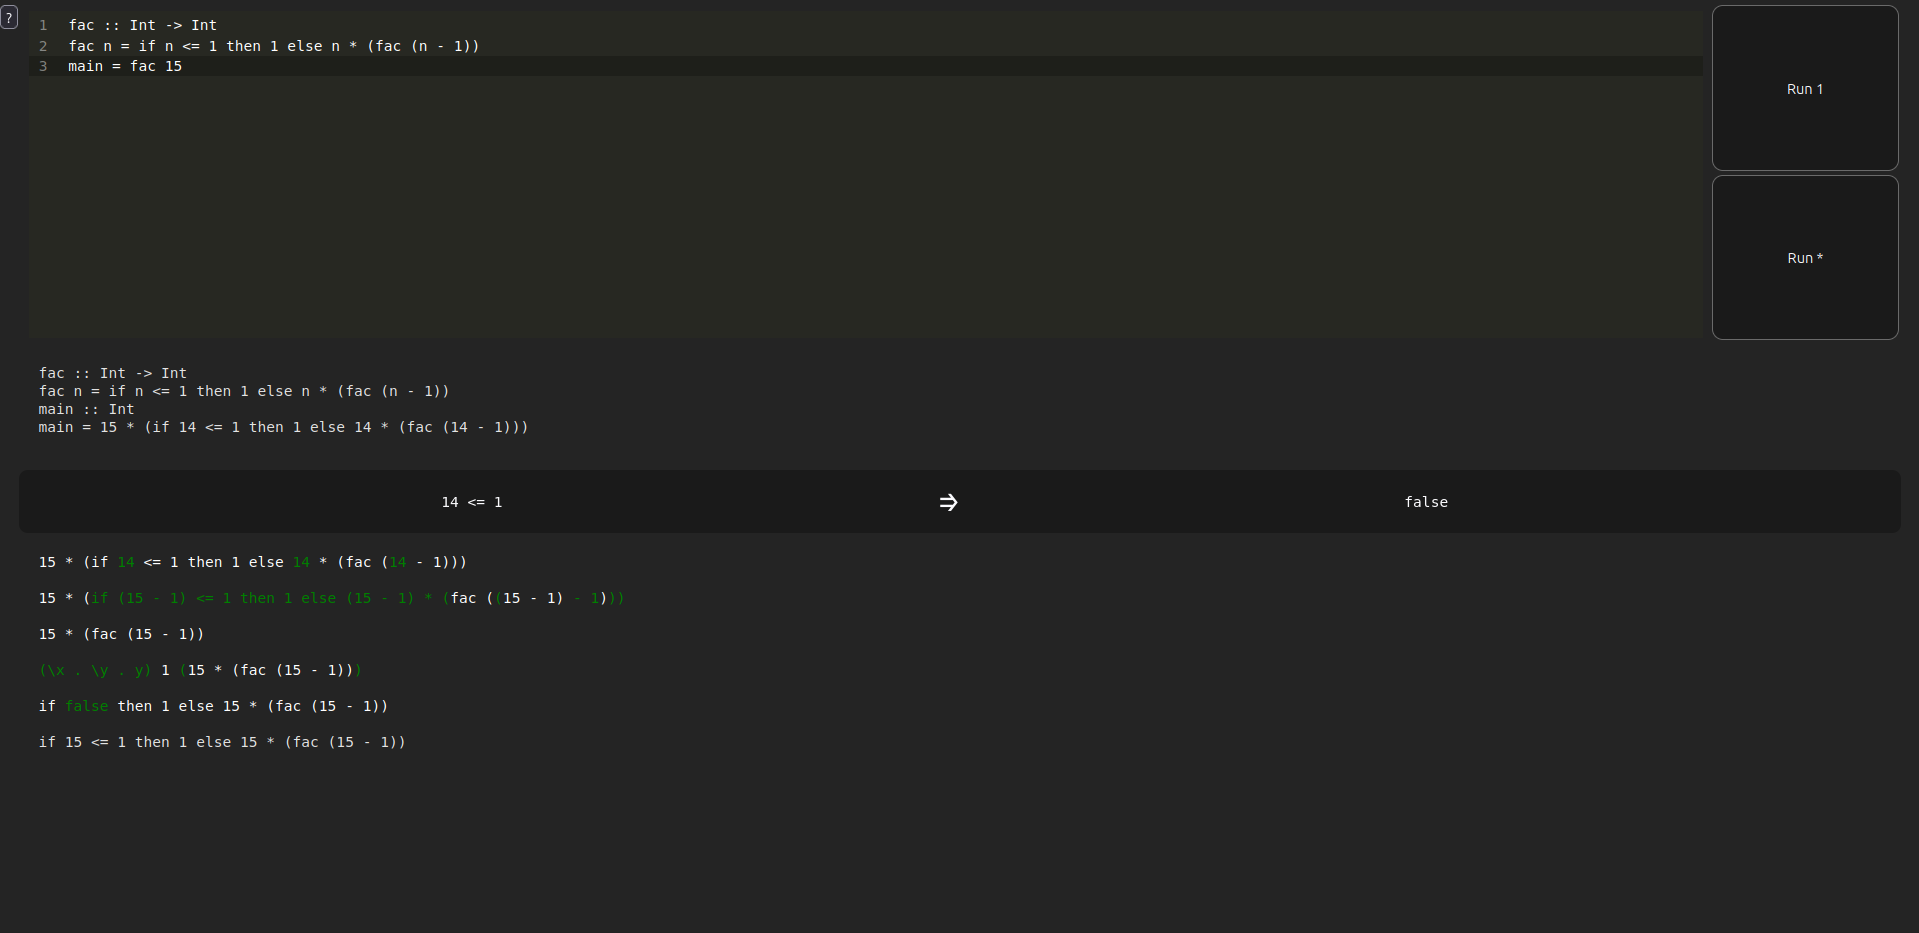
\includegraphics[width=1\linewidth]{images/product_at_testathon.png}
    \caption{The UI as tested in the testathon}
    \label{fig:screenshot_testathon}
\end{figure}

\begin{figure}
    \centering
    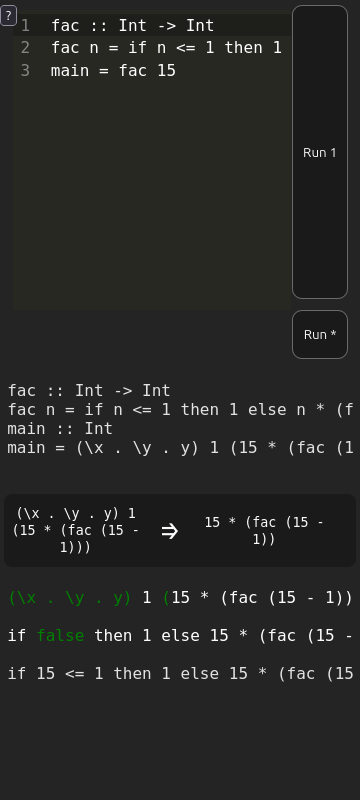
\includegraphics[width=0.5\linewidth]{images/testathon-mobile.png}
    \caption{The UI as tested in the testathon, as it would have appeared on a Samsung Galaxy S20}
    \label{fig:screenshot_testathon_mobile}
\end{figure}

\begin{figure}
    \centering
    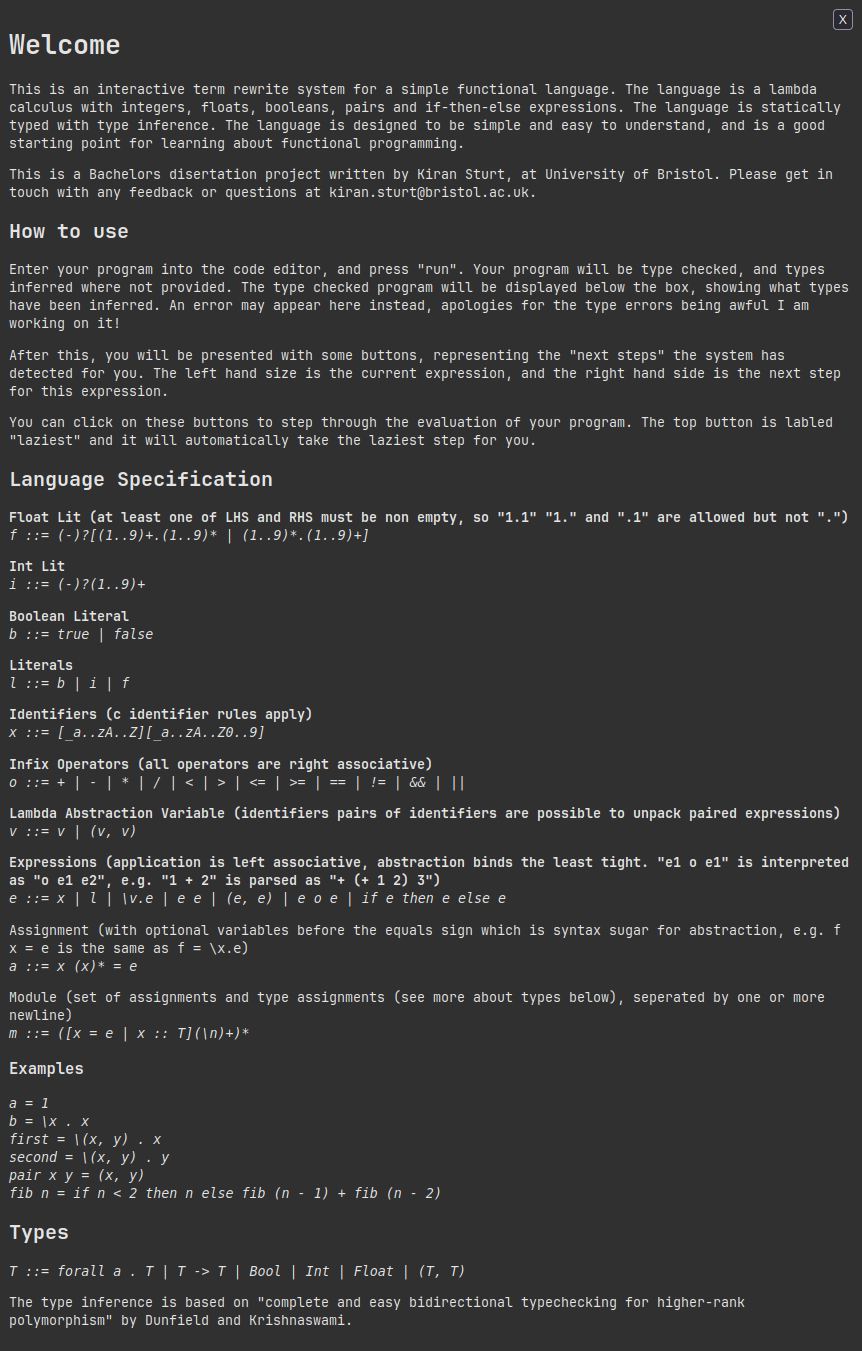
\includegraphics[width=0.9\linewidth]{images/testathon_help_menu_cropped.png}
    \caption{The "Help menu" in the testathon. This was spawned by pressing the "?" button in the top left of the UI, and dismissed by pressing the "X" button, or clicking outside of the box}
    \label{fig:screenshot_testathon_2}
\end{figure}

\chapter{Type System}
\def\OPTIONConf{1}
\linespread{1}

\renewcommand{\mathstrut}{\rule[-1pt]{0pt}{2pt}}

\def\OPTIONLoudLabels{0}
\def\OPTIONArxiv{1}

\definecolor{dHilite}{rgb}{0.9, 0.9, 0.6}
\definecolor{dRed}{rgb}{0.65, 0.0, 0.0}
\definecolor{dGreen}{rgb}{0.0, 0.65, 0.0}
\definecolor{dDkGreen}{rgb}{0.0, 0.35, 0.0}
\definecolor{dBlue}{rgb}{0.0, 0.0, 0.65}
\definecolor{dPurple}{rgb}{0.65, 0.0, 0.65}
\definecolor{dDigPurple}{rgb}{0.5, 0.0, 0.5}
\definecolor{dFaint}{rgb}{0.7, 0.7, 0.7}
\definecolor{dGray}{rgb}{0.5, 0.5, 0.5}
\definecolor{dDark}{rgb}{0.2, 0.2, 0.2}
\definecolor{dAlmostBlack}{rgb}{0.1, 0.1, 0.1}

\makeatletter
\def\url@MGstyle{%
\def\UrlFont{\tiny\huge\ttfamily}%
%
%
\Url@do
}
\makeatother
%
%
\newcommand{\marginPseudoURL}[1]{\tt #1}
\newcommand{\marginnote}[1]{\marginparwidth=40pt \marginpar{%
    \raisebox{-2ex}{\parbox{40pt}{\raggedright\scriptsize #1}}}}

\makeatletter
\def\url@vttstyle{%
  \@ifundefined{selectfont}{\def\UrlFont{\tt}}{\def\UrlFont{\normalfont\fontfamily{cmvtt}\selectfont}}}
\makeatother
%
\urlstyle{vtt}

%
%
%
%
%
%

\newcommand\textvtt[1]{{\normalfont\fontfamily{cmvtt}\selectfont #1}}

\newcommand{\LoudLabel}[1]{\idempotentlabel{#1}%
\ifnum\OPTIONLoudLabels=1%
  \ifnum\OPTIONConf=1%
  \marginnote{\tiny\textvtt{#1}}%
  \else%
  \marginnote{\textvtt{#1}}%
  \fi%
\fi%
}

\newcommand{\idempotentlabel}[1]{%
    \ifcsname IDEMPFLAG#1\endcsname%
      %
      \message{YYY ALREADY DEFINED: #1}
    \else%
      %
      \message{YYZ NOT ALREADY DEFINED: #1}
      \expandafter\gdef\csname IDEMPFLAG#1\endcsname{d}%
      %
      \label{#1}%
    \fi}

%

%
\ifnum\OPTIONLoudLabels=1%
\newcommand{\Label}[1]{\LoudLabel{#1}}%
\newcommand{\FLabel}[1]{\idempotentlabel{#1}%
{\tt\scriptsize{#1}}}%
\else%
\newcommand{\Label}[1]{\idempotentlabel{#1}}%
\newcommand{\FLabel}[1]{\idempotentlabel{#1}}%
\fi

%
%
%
%
%
%
%
%
\newdimen\zzfontsz
\newcommand{\fontsz}[2]{\zzfontsz=#1%
{\fontsize{\zzfontsz}{1.2\zzfontsz}\selectfont{#2}}}

\newcommand{\texfontsz}[1]{\zzfontsz=#1%
\fontsize{\zzfontsz}{1.25\zzfontsz}\selectfont}

\newcommand{\mathsz}[2]{\text{\fontsz{#1}{$#2$}}}

\newcommand{\XX}{\text{\ding{55}}}
\newcommand{\redXX}{\text{\textcolor{dRed}{\XX}}}
\newcommand{\greencheck}{\text{\textcolor{dGreen}{\checkmark}}}

\newcommand{\fixme}[1]{\textcolor{red}{\texttt{FIXME: {#1}}}}

\newcommand{\flaming}[1]{\textcolor{red}{\fontsz{18pt}{\bf #1}}}
\newcommand{\flamingmath}[1]{\textcolor{red}{\fontsz{18pt}{\bf \ensuremath{#1}}}}

\newcommand{\semiflaming}[1]{\textcolor{dRed}{\sl #1}}

% \newcommand{\mathcolor}[2]{\text{\textcolor{#1}{\ensuremath{#2}}}}

%
\newcommand{\smallblacktriangle}{\text{\textscale{0.7}{$\blacktriangleright$}}}

\newcommand{\setof}[1]{\left\{#1\right\}}
\newcommand{\comprehend}[2]{\setof{{#1} \;\middle|\; {#2}}}

\newcommand{\assign}{\ensuremath{\,{:=}\,}}

\newcommand{\arr}{\rightarrow}
%
%
\def\CompactJudgments{0}
\newcommand{\entails}{\mathrel{\ifnum\CompactJudgments=1%
    \vdash%
  \else%
     \vdash\,%
  \fi}}
\newcommand{\ctxoutsym}{\ifnum\CompactJudgments=1%
    \dashv%
  \else%
     \,\dashv%
  \fi}
\newcommand{\ctxout}[1]{\mathrel{\ctxoutsym}{#1}}

%
\newcommand{\J}{\mathcal{J}}
\newcommand{\judg}{\J}

\newcommand{\MonnierCommaSym}{{\smallblacktriangle}}
\newcommand{\MonnierComma}[1]{{\MonnierCommaSym}_{#1}}

\newcommand{\FV}[1]{\mathrm{FV}(#1)}
\newcommand{\xfev}{\mathsf{FEV}}
\newcommand{\fev}[1]{\xfev(#1)}
\newcommand{\FEV}[1]{\fev{#1}}
\newcommand{\xfsolev}{\mathsf{FSolEV}}
\newcommand{\fsolev}[2]{\xfsolev_{#1}(#2)}

\newcommand{\beeq}{=_{\beta\eta}}

\newcommand{\kindstar}{\star}
\newcommand{\kindnat}{\mathbb{N}}

\newcommand{\inversefn}[1]{{#1}^{-1}}

\newcommand{\emptysig}{\cdot}
\newcommand{\emptyctx}{\cdot}

\newcommand{\natzero}{\mathsf{zero}}
\newcommand{\xnatsucc}{\mathsf{succ}}
\newcommand{\natsucc}[1]{\xnatsucc\texttt{(}{#1}\texttt{)}}


\newcommand{\instantiate}[1]{{#1}\texttt{[-]}}
\newcommand{\quantify}[1]{\Lambda{#1}.\,}


\newcommand{\exvar}[1]{\widehat{#1}}
\newcommand{\exalpha}{\exvar{\alpha}}
\newcommand{\exbeta}{\exvar{\beta}}

\newcommand{\alln}[1]{\forall{#1}{:}\kindnat.\,}

\newcommand{\Match}[2]{{#1} \Rightarrow {#2}}
\newcommand{\matchor}{\ensuremath{\normalfont\,\texttt{|}\hspace{-5.35pt}\texttt{|}\,}}
\newcommand{\ind}[3]{\mathsf{ind}\texttt{(}\Match{\natzero}{#1}%
                     \texttt{,\;}%
                     \Match{\natsucc{#2}}{#3}
                     \texttt{)}}

\newcommand{\exunk}[2]{{#1} : {#2}}
\newcommand{\exsol}[3]{{#1} : {#2} \texttt{=} {#3}}
\newcommand{\exsolnokind}[2]{{#1} \texttt{=} {#2}}
\newcommand{\exsolwild}[2]{({#1} : {#2}\dots)}
\newcommand{\rexvar}[2]{\exsolnokind{#1}{#2}}

\newcommand{\tyname}[1]{\textsf{\normalfont #1}}
%
\newcommand{\unitexp}{\text{\normalfont \tt()}}
\newcommand{\unitty}{\tyname{1}}

\newcommand{\trientails}{\mathrel{{\rhd}\,}}
\newcommand{\trictxoutsym}{{\lhd}}
\newcommand{\trictxout}[1]{\mathrel{\trictxoutsym}{#1}}

\newcommand{\subtypingycolor}[1]{\textcolor{dDigPurple}{#1}}
%
\newcommand{\subtype}{\mathrel{\normalfont\texttt{\subtypingycolor{<:}}}}  %
\newcommand{\declsubtype}{\mathrel{\leq}}

\newcommand{\etal}{{et al.}}
\newcommand{\eg}{e.g.\ }
\newcommand{\ie}{i.e.\ }
\newcommand{\ala}{\`a la\ }
\newcommand{\Wlog}{w.l.o.g.\ }
\newcommand{\visavis}{vis-\`a-vis\ }
\newcommand{\Ocaml}{{OCaml}\xspace}
\newcommand{\OCaml}{\Ocaml}

\newcommand{\naive}{na\"ive\xspace}
\newcommand{\Backslash}{\char"5C}
\newcommand{\Lbrack}{\char"5B}
\newcommand{\Rbrack}{\char"5D}
\newcommand{\Lbrace}{\char"7B}
\newcommand{\Rbrace}{\char"7D}

\newcommand{\Appendixref}[1]{Appendix \ref{#1}}
\newcommand{\Figureref}[1]{Figure \ref{#1}}
\newcommand{\Figref}[1]{Fig.\ \ref{#1}}
\newcommand{\Sectionref}[1]{Section \ref{#1}}
\newcommand{\Secref}[1]{Sec.\ \ref{#1}}
\newcommand{\Chapterref}[1]{Chapter \ref{#1}}

\newcommand{\Listingref}[1]{Listing \ref{#1}}

\newcommand{\Theoremref}[1]{Theorem \ref{#1}}
\newcommand{\Thmref}[1]{Thm.\ \ref{#1}}
\newcommand{\Corollaryref}[1]{Corollary \ref{#1}}
\newcommand{\Corref}[1]{Cor.\ \ref{#1}}
\newcommand{\Lemmaref}[1]{Lemma \ref{#1} (\nameref{#1})}   %
\newcommand{\Lemref}[1]{\Lemma \ref{#1}}   %
%
\newcommand{\Conjectureref}[1]{Conjecture \ref{#1}}
\newcommand{\Propositionref}[1]{Proposition \ref{#1}}
\newcommand{\Propertyref}[1]{Property \ref{#1}}
\newcommand{\Remarkref}[1]{Remark \ref{#1}}
\newcommand{\Tableref}[1]{Table \ref{#1}}

\newcommand{\Definitionref}[1]{Definition \ref{#1}}
\newcommand{\Defnref}[1]{Def.\ \ref{#1}}

%
\newcommand{\ProofCaseRule}[1]{\item \textbf{Case }\textrm{{#1}}: ~ }
\newcommand{\ProofCaseThing}[1]{\ProofCaseRule{\ensuremath{#1}}}
\newcommand{\ProofCasesRules}[1]{\item \textbf{Cases }\textrm{{#1}}: ~ }
\newcommand{\ProofCaseRuleNoColon}[1]{\item \textbf{Case }\textrm{{#1}}}

\gdef\xxDerivationProofCaseColor{N}
\newcommand{\Begincolorcases}[1]{\gdef\xxDerivationProofCaseColor{#1}}
\newcommand{\Endcolorcases}{\gdef\xxDerivationProofCaseColor{N}}

%
%
%
%
%
%
%
%
%
%
%
%
%
%
%
%
%
%
%
%
%
%
%
\newcommand{\DerivationProofCase}[3]{%
     \smallskip
     \item %
       \parbox[t]{100ex}{%
       \textbf{Case } \\[-0.5em]
       $~$\hspace{5ex}
       \if\xxDerivationProofCaseColor N%
           \ensuremath{%
              \Infer{#1}{#2}{#3}%
            }
       \else%
           \colorbox{\xxDerivationProofCaseColor}{%
              \ensuremath{%
                \Infer{#1}{#2}{#3}%
              }%
           }%
        \fi%
     }%
     \nopagebreak \\[-0.8ex]
  }

\newcommand{\DoubleDerivationProofCase}[6]{%
     \smallskip
     \item %
       \parbox[t]{100ex}{%
       \textbf{Case } \\[-0.5em]
       $~$\hspace{5ex}
       \if\xxDerivationProofCaseColor N%
           \ensuremath{%
              \Infer{#1}{#2}{#3}%
              ~~~~~
              \Infer{#4}{#5}{#6}%
            }
       \else%
           \colorbox{\xxDerivationProofCaseColor}{%
              \ensuremath{%
                \Infer{#1}{#2}{#3}%
                ~~~~~
                \Infer{#4}{#5}{#6}%
              }%
           }%
        \fi%
     }%
     \nopagebreak \\[-0.8ex]
  }

\newcommand{\Dee}{\mathcal{D}}
\newcommand{\D}{\mathcal{\Dee}}

\newenvironment{displ}{\vspace{1pt} \begin{center} ~\!\!}{\end{center}}
\newenvironment{mathdispl}{\vspace{1pt} \begin{center} ~\!\!\(}{\)\end{center}}

\newenvironment{ctabular}{%
      \renewcommand{\arraystretch}{1}%
         \vspace{1pt}%
         \begin{center} ~\!\!%
           \begin{tabular}[t]{l}%
     }{%
            \end{tabular}%
          \end{center}%
      }

\newcommand{\arrayenv}[1]{\renewcommand{\arraystretch}{1} \begin{array}[t]{@{}c@{}}#1\end{array}}
\newcommand{\arrayenvc}[1]{\renewcommand{\arraystretch}{1} \begin{array}[c]{@{}c@{}}#1\end{array}}
\newcommand{\arrayenvcl}[1]{\renewcommand{\arraystretch}{1} \begin{array}[c]{@{}l@{}}#1\end{array}}
\newcommand{\arrayenvr}[1]{\renewcommand{\arraystretch}{1} \begin{array}[t]{@{}r@{}}#1\end{array}}
\newcommand{\arrayenvbr}[1]{\renewcommand{\arraystretch}{1} \begin{array}[b]{@{}r@{}}#1\end{array}}
\newcommand{\arrayenvl}[1]{\renewcommand{\arraystretch}{1} \begin{array}[t]{@{}l@{}}#1\end{array}}
\newcommand{\arrayenvb}[1]{\renewcommand{\arraystretch}{1}  \begin{array}[b]{@{}c@{}}#1\end{array}} 
\newcommand{\arrayenvbl}[1]{\renewcommand{\arraystretch}{1}  \begin{array}[b]{@{}l@{}}#1\end{array}}
\newcommand{\arrayenvblll}[1]{\renewcommand{\arraystretch}{1}  \begin{array}[b]{@{}lll@{}}#1\end{array}}
\newcommand{\pfarr}[1]{\begin{array}[b]{@{}l@{}}#1\end{array}}

%
\newcommand{\BeginProof}{\renewcommand{\arraystretch}{1.1} \begin{tabular}[b]{r@{}r @{} l  l}}
\newcommand{\EndProof}{\end{tabular} \renewcommand{\arraystretch}{\mydefaultarraystretch}}

\newcommand{\Hand}{\text{\Pointinghand~~~~}}

\newcommand{\Pf}[4] {&$#1$ $#2$\, & $#3$ & #4 \\}
\newcommand{\Pfmrg}[3] {&$#1$\, & $#2$ & #3 \\}
\newcommand{\stepPf}[3] {\Pf{#1}{\,\step\,}{#2}{#3}}
\newcommand{\EPf}[3] {\Pf{#1}{\Entails}{#2}{#3}}
\newcommand{\LetPf}[3] {\Pf{\text{Let}\,~{#1}}{=\,}{#2\text{.}}{#3}}
\newcommand{\ForallPf}[3] {\Pf{\text{For all}\,~{#1}}{\in\,}{#2}{#3}}
\newcommand{\mkpf}[4] {\Pf{#2}{#1\,}{#3}{#4}}

\newcommand{\ePf}[3] {\mkpf{\entails}{#1}{#2}{#3}}
\newcommand{\eqPf}[3] {\mkpf{=}{#1}{#2}{#3}}
\newcommand{\continueeqPf}[2] {\mkpf{=}{~}{#1}{#2}}
\newcommand{\rightstarteqPf}[1] {\mkpf{~}{~}{#1}{~}}
\newcommand{\neqPf}[3] {\mkpf{\neq}{#1}{#2}{#3}}
\newcommand{\ltPf}[3] {\mkpf{<}{#1}{#2}{#3}}
\newcommand{\leqPf}[3] {\mkpf{\leq}{#1}{#2}{#3}}
\newcommand{\inPf}[3] {\mkpf{\in}{#1}{#2}{#3}}
\newcommand{\notinPf}[3] {\mkpf{\notin}{#1}{#2}{#3}}

\newcommand{\trailingjust}[1]{\Pf{}{}{}{~~{#1}}}
\newcommand{\derivesPf}[1]{${#1} \derives~~$}

\newcommand{\contraPf}[1] {%
          \Pf{\Rightarrow\Leftarrow}{}{} {}%
          \Pf{#1}{}{} {By contradiction}%
       }

\newcommand{\NOTePf}[3] {\Pf{#1}{\not\entails\;}{#2}{#3}}
\newcommand{\proofsep}{\,\\[-0.5em]}
\newcommand{\PfTwo}[7]{\Pf{\arrayenvr{{#1}\\{#4}}}{\arrayenvl{{#2}\\{#5}}}{\arrayenvl{{#3}\\{#6}}}%
                                              {\drophalf{\!\ensuremath{\left\} \begin{array}{r l} \,\\ \, \end{array}\!\!\!\!\!%
                                                      \text{#7} \right.}}}}
\newenvironment{llproof}{\BeginProof}{\EndProof}
\newcommand{\decolumnizePf}{\end{llproof} ~\\ \begin{llproof}}

%
\newcommand{\proofheading}[1]{}  %

\newcommand{\ditto}{\ensuremath{''}}


\newcommand{\xdom}{\mathsf{dom}}
\newcommand{\dom}[1]{\xdom(#1)}

\newcommand{\xweight}{\mathsf{weight}}
\newcommand{\weight}[2]{\xweight_{#1}(#2)}

\newcommand{\xangst}{\mathsf{angst}}
\newcommand{\angst}[2]{\xangst_{#1}(#2)}

\newcommand{\xunsol}{\mathsf{unsol}}
\newcommand{\unsol}[2]{\xunsol_{#1}(#2)}

\newcommand{\xunsolved}{\mathsf{unsolved}}
\newcommand{\unsolved}[1]{\xunsolved(#1)}

\newcommand{\xGtypesize}[1]{\mathsf{size}_{#1}}
\newcommand{\Gtypesize}[2]{\xGtypesize{#1}(#2)}

\newcommand{\union}{\mathrel{\cup}}
\newcommand{\sect}{\mathrel{\cap}}


\newcommand{\normalize}{\mathrel{\Downarrow}}


%
%
\newcommand{\textgraybox}[1]{\boxed{#1}}
\newcommand{\graybox}[1]{\textgraybox{\ensuremath{#1}}}

\newcommand{\tightcolorbox}[2]{\setlength{\fboxsep}{1pt}\colorbox{#1}{#2}}

%
\newcommand{\textcolorbox}[2]{\tightcolorbox{#1}{#2}}
\newcommand{\textshadebox}[1]{\textcolorbox{grayboxgray}{#1}}
%
\newcommand{\shadebox}[1]{\text{\textshadebox{\ensuremath{#1}}}}

%

%
\newcommand{\mathcolorbox}[2]{\text{\tightcolorbox{#1}{$\displaystyle {#2}$}}}

%
%
%
%

\newcommand{\judgboxfontsize}[1]{%
    \ifnum\OPTIONConf=1%
        \mathsz{11pt}{#1}%
    \else%
        \mathsz{14pt}{#1}%
    \fi}
\newcommand{\judgbox}[2]{%
      {\raggedright \textgraybox{\ensuremath{\judgboxfontsize{#1}}}\!%
        \fontsz{9pt}{\begin{tabular}[c]{l} #2 \end{tabular}} %
}}


\newcommand{\bnfas}{\mathrel{::=}}
\newcommand{\bnfalt}{\mathrel{\mid}}

\newcommand{\derives}{\mathrel{::}}

\newcommand{\AllSym}{\forall}
\newcommand{\xAll}[1]{\AllSym#1}
\newcommand{\All}[1]{\xAll{#1}.\:}

\newcommand{\AND}{\text{~~and~~}}

\newcommand{\Infer}[3]{\inferrule*[right={\text{\strut#1}}]{{}#2\mathstrut}{{}#3\mathstrut}}




\newcommand{\keyword}[1]{\textsf{#1}}
\newcommand{\textkw}[1]{\keyword{#1}}
\newcommand{\lam}[1]{\lambda #1.\,}
\newcommand{\fun}[2]{\lam{#1}{#2}}
\newcommand{\typelam}[1]{\Lambda #1.\,}
\newcommand{\LAM}[1]{\typelam{#1}}
\newcommand{\Let}[2]{\textkw{let}\;{#1}\,\texttt{=}\,{#2}\;\textkw{in}\;}

\newcommand{\bigprec}{\mathrel{\mathsz{14pt}{\prec}}}


\newcommand{\atomic}[1]{{#1}\;\mathrm{atomic}}

\newcommand{\declsubjudg}[3]{\ensuremath{{#1} \entails {#2} \declsubtype {#3}}}
\newcommand{\typejudg}[3]{\ensuremath{{#1} \entails {#2} : {#3}}}
\newcommand{\subjudg}[4]{\ensuremath{{#1} \entails {#2} \subtype {#3} \ctxout{#4}}}

%
%
\newdimen\zzinstsymLTwidth
\newdimen\zzinstsymEQwidth
\newdimen\zzinstsymDiff
\newcommand{\instsymLeq}{%
    \settowidth{\zzinstsymLTwidth}{\text{\normalfont\tt<}}%
    \settowidth{\zzinstsymEQwidth}{\text{\normalfont=}}%
    \setlength{\zzinstsymDiff}{\zzinstsymEQwidth}%
    \addtolength{\zzinstsymDiff}{-\zzinstsymLTwidth}%
    \text{\raisebox{-0.22ex}{\normalfont=}%
%
    \hspace{-\zzinstsymEQwidth}%
    \hspace{0.5\zzinstsymDiff}%
    \raisebox{0.77ex}{\normalfont\tt<}}}
\newcommand{\instsymColon}{%
     \raisebox{-0.09ex}{\text{\normalfont{:}}}}
%
%
%
\newcommand{\instsyml}{\subtypingycolor{\instsymColon\hspace{0.05ex}\instsymLeq}}
\newcommand{\instsymr}{\subtypingycolor{\instsymLeq\hspace{0.05ex}\instsymColon}}
\newcommand{\instsymlop}{\mathrel{\instsyml}}
\newcommand{\instsymrop}{\mathrel{\instsymr}}

\newcommand{\instjudg}[4]{\ensuremath{{#1} \entails {#2} \instsymlop {#3} \ctxout{#4}}}
\newcommand{\instjudgr}[4]{\ensuremath{{#1} \entails {#3} \instsymrop {#2} \ctxout{#4}}}

\newcommand{\declsubjudgPf}[4] {\Pf{#1}{\entails}{{#2} \declsubtype {#3}}{#4}}
\newcommand{\subjudgPf}[5] {\Pf{#1}{\entails}{{#2} \subtype {#3} \ctxout{#4}}{#5}}
\newcommand{\substextendPf}[3] {\Pfmrg{{#1} \extendssym\,}{#2}{#3}}
\newcommand{\instjudgPf}[5]{\Pf{#1}{\entails}{{#2} {\;\instsyml\;} {#3} \ctxout{#4}}{#5}}
\newcommand{\instjudgrPf}[5]{\Pf{#1}{\entails}{{#3} {\;\instsymr\;} {#2} \ctxout{#4}}{#5}}

\newcommand{\chkcolor}{dBlue}
\newcommand{\syncolor}{dRed}
\newcommand{\appcolor}{dDkGreen}
\newcommand{\chk}{\mathrel{\mathcolor{\chkcolor}{\Leftarrow}}}
\newcommand{\uncoloredsyn}{{\Rightarrow}}
\newcommand{\syn}{\mathrel{\mathcolor{\syncolor}{\uncoloredsyn}}}
\newcommand{\appsep}{\;{\mathcolor{\appcolor}{\bullet}}\;}
%
\newcommand{\app}{\mathrel{\mathcolor{\appcolor}{{\uncoloredsyn}\hspace{-1.2ex}{\uncoloredsyn}}}}

\newcommand{\chkjudg}[4]{\ensuremath{{#1} \entails {#2} \chk {#3} \ctxout{#4}}}
\newcommand{\appjudg}[5]{\ensuremath{{#1} \entails {#3} \appsep {#2} \app {#4} \ctxout{#5}}}
\newcommand{\synjudg}[4]{\ensuremath{{#1} \entails {#2} \syn {#3} \ctxout{#4}}}

\newcommand{\declchkjudg}[3]{\ensuremath{{#1} \entails {#2} \chk {#3}}}
\newcommand{\declappjudg}[4]{\ensuremath{#1} \entails {#3} \appsep {#2}  \app {#4}}
\newcommand{\declsynjudg}[3]{\ensuremath{{#1} \entails {#2} \syn {#3}}}

\newcommand{\chkjudgPf}[5]{\Pf{#1}{\entails}{{#2} \chk {#3} \ctxout{#4}}{#5}}
\newcommand{\appjudgPf}[6]{\Pf{#1}{\entails}{{#3} \appsep {#2} \app {#4} \ctxout{#5}}{#6}}
\newcommand{\synjudgPf}[5]{\Pf{#1}{\entails}{{#2} \syn {#3} \ctxout{#4}}{#5}}
\newcommand{\declchkjudgPf}[4]{\Pf{#1}{\entails}{{#2} \chk {#3}}{#4}}
\newcommand{\declappjudgPf}[5]{\Pf{#1}{\entails}{{#3} \appsep {#2} \app {#4}}{#5}}
\newcommand{\declsynjudgPf}[4]{\Pf{#1}{\entails}{{#2} \syn {#3}}{#4}}


\newcommand{\hyp}[2]{{#1}:{#2}}
\newcommand{\hypeq}[2]{{#1} = {#2}}
\newcommand{\tighthypeq}[2]{{#1}{=}{#2}}
%
\newcommand{\alltype}[1]{\All{#1}}
\newcommand{\num}{\mathsf{int}}
\newcommand{\bool}{\mathsf{bool}}

\newcommand{\grow}[2]{{#1} \sqsupseteq {#2}}

\newcommand{\idsubst}{\mathsf{id}}

\newcommand{\extendssym}{\longrightarrow}
\newcommand{\extends}[2]{{#1} \extendssym {#2}}
%
\newcommand{\substextend}[2]{\extends{#1}{#2}}

\newcommand{\judgetp}[2]{{#1} \entails {#2}}
\newcommand{\judgetpPf}[3]{\Pf{#1}{\entails}{#2}{#3}}
%
%
\newcommand{\typesize}[2]{|{#1} {\;\entails} {#2}|}

\newcommand{\judgectx}[1]{{#1}~\mathit{ctx}}
\newcommand{\judgectxPf}[2]{\Pf{}{}{\judgectx{#1}}{#2}}

\newcommand{\xcompletes}{\ensuremath{\mathsf{completes}}}
\newcommand{\xcompletedby}{\ensuremath{\mathsf{completed\;by}}}
%
\newcommand{\completedby}[2]{{#1} \;\flamingmath{\xcompletedby}\; {#2}}
\newcommand{\apply}[2]{{[{#1}]}{#2}}

\newcommand{\ahat}{\hat{\alpha}}
\newcommand{\bhat}{\hat{\beta}}
\newcommand{\chat}{\hat{\gamma}}
\newcommand{\dhat}{\hat{\delta}}

%
%
%
\newcommand{\hsubst}[5]{[{#2}/{#3}]^{#1}_{#2}{#4}}

%
%
%
\newcommand{\rulename}[1]{\text{\normalfont\textsf{#1}}}

%
%
%
\newcommand{\substextendrulename}[1]{\ensuremath{{\extendssym}{\rulename{#1}}}\xspace}
\newcommand{\substextendId}{\substextendrulename{ID}}

\newcommand{\substextendUU}{\substextendrulename{Uvar}}
\newcommand{\substextendVV}{\substextendrulename{Var}}
\newcommand{\substextendEE}{\substextendrulename{Unsolved}}
\newcommand{\substextendSolSol}{\substextendrulename{Solved}}
\newcommand{\substextendMonMon}{\substextendrulename{Marker}}

\newcommand{\substextendSolve}{\substextendrulename{Solve}}
\newcommand{\substextendAdd}{\substextendrulename{Add}}
\newcommand{\substextendAddSolved}{\substextendrulename{AddSolved}}


%
%
%
\newcommand{\Dsubrulename}[1]{\ensuremath{{\declsubtype}\rulename{#1}}\xspace}
\newcommand{\DsubVar}{\Dsubrulename{Var}}
\newcommand{\DsubUnit}{\Dsubrulename{Unit}}
\newcommand{\DsubArr}{\Dsubrulename{\ensuremath{\arr}}}
\newcommand{\DsubImp}{\DsubArr} %
\newcommand{\DsubAllL}{\Dsubrulename{\ensuremath{\forall}{L}}}
\newcommand{\DsubAllR}{\Dsubrulename{\ensuremath{\forall}{R}}}

%
%
%
\newcommand{\Subrulename}[1]{\ensuremath{{\subtype}\rulename{#1}}\xspace}
\newcommand{\SubVar}{\Subrulename{Var}}
\newcommand{\SubUnit}{\Subrulename{Unit}}
\newcommand{\SubExvar}{\Subrulename{Exvar}}
\newcommand{\SubArr}{\Subrulename{\ensuremath{\arr}}}
\newcommand{\SubImp}{\SubArr} %
\newcommand{\SubAllL}{\Subrulename{\ensuremath{\forall}{L}}}
\newcommand{\SubAllR}{\Subrulename{\ensuremath{\forall}{R}}}

\newcommand{\SubSubst}[1]{\Subrulename{\flaming{Subst{#1}}}}
\newcommand{\SubSubstL}{\SubSubst{L}}
\newcommand{\SubSubstR}{\SubSubst{R}}

\newcommand{\SubInst}[1]{\Subrulename{Instantiate{#1}}}
\newcommand{\SubInstL}{\SubInst{L}}
\newcommand{\SubInstR}{\SubInst{R}}

%
%
%
\newcommand{\DeclWFrulename}[1]{\ensuremath{\rulename{Decl{#1}WF}}\xspace}
\newcommand{\DeclUvarWF}{\DeclWFrulename{Uvar}}
\newcommand{\DeclUnitWF}{\DeclWFrulename{Unit}}
\newcommand{\DeclArrowWF}{\DeclWFrulename{Arrow}}
\newcommand{\DeclForallWF}{\DeclWFrulename{Forall}}

%
%
%
\newcommand{\WFrulename}[1]{\ensuremath{\rulename{{#1}WF}}\xspace}
\newcommand{\UvarWF}{\WFrulename{Uvar}}
\newcommand{\UnitWF}{\WFrulename{Unit}}
\newcommand{\EvarWF}{\WFrulename{Evar}}
\newcommand{\SolvedEvarWF}{\WFrulename{SolvedEvar}}
\newcommand{\ArrowWF}{\WFrulename{Arrow}}
\newcommand{\ForallWF}{\WFrulename{Forall}}


%
%
%
\newcommand{\CWFrulename}[1]{\ensuremath{\rulename{{#1}Ctx}}\xspace}
\newcommand{\EmptyCWF}{\CWFrulename{Empty}}
\newcommand{\UvarCWF}{\CWFrulename{Uvar}}
\newcommand{\EvarCWF}{\CWFrulename{Evar}}
\newcommand{\SolvedEvarCWF}{\CWFrulename{SolvedEvar}}
\newcommand{\VarCWF}{\CWFrulename{Var}}
\newcommand{\MarkerCWF}{\CWFrulename{Marker}}


%
%
%
\newcommand{\Instrulename}[1]{\ensuremath{\rulename{Inst{#1}}}\xspace}
\newcommand{\InstLrulename}[1]{\Instrulename{L{#1}}}
\newcommand{\InstRrulename}[1]{\Instrulename{R{#1}}}

\newcommand{\InstLSolve}{\InstLrulename{Solve}}
\newcommand{\InstLReach}{\InstLrulename{Reach}}
\newcommand{\InstLArr}{\InstLrulename{Arr}}
\newcommand{\InstLAllR}{\InstLrulename{AllR}}

\newcommand{\InstRSolve}{\InstRrulename{Solve}}
\newcommand{\InstRReach}{\InstRrulename{Reach}}
\newcommand{\InstRArr}{\InstRrulename{Arr}}
\newcommand{\InstRAllL}{\InstRrulename{AllL}}


%
%
%
\newcommand{\CompletesRule}{\rulename{completes}}
%
%
%
%
%
%
%
%




%
%
%
\newcommand{\Decltyrulename}[1]{\ensuremath{\rulename{Decl#1}}\xspace}

\newcommand{\DeclIntrorulename}[1]{\Decltyrulename{\ensuremath{#1}I}}
\newcommand{\DeclIntroSynrulename}[1]{\Decltyrulename{\ensuremath{#1}I$\syn$}}
\newcommand{\DeclElimrulename}[1]{\Decltyrulename{\ensuremath{#1}E}}
\newcommand{\DeclApprulename}[1]{\Decltyrulename{\ensuremath{#1}App}}

%
\newcommand{\DeclVar}{\Decltyrulename{Var}}
\newcommand{\DeclSub}{\Decltyrulename{Sub}}
\newcommand{\DeclAnno}{\Decltyrulename{Anno}}

%
\newcommand{\DeclUnitIntro}{\DeclIntrorulename{\unitty}}
%
\newcommand{\DeclUnitIntroSyn}{\DeclIntroSynrulename{\unitty}}

%
\newcommand{\DeclArrIntro}{\DeclIntrorulename{\arr}}
\newcommand{\DeclArrIntroSyn}{\DeclIntroSynrulename{\arr}}
\newcommand{\DeclArrElim}{\DeclElimrulename{\arr}}

%
\newcommand{\DeclAllIntro}{\DeclIntrorulename{\AllSym}}
%
\newcommand{\DeclAllElim}{\DeclElimrulename{\AllSym}}

\newcommand{\DeclArrApp}{\DeclApprulename{\arr}}
%
\newcommand{\DeclAllApp}{\DeclApprulename{\forall}}
%

%
%
%
\newcommand{\Tyrulename}[1]{\ensuremath{\rulename{#1}}\xspace}

\newcommand{\Introrulename}[1]{\Tyrulename{\ensuremath{#1}I}}
\newcommand{\IntroSynrulename}[1]{\Tyrulename{\ensuremath{#1}I$\syn$}}
\newcommand{\Elimrulename}[1]{\Tyrulename{\ensuremath{#1}E}}
\newcommand{\Apprulename}[1]{\Tyrulename{\ensuremath{#1}App}}

%
\newcommand{\Var}{\Tyrulename{Var}}
\newcommand{\Sub}{\Tyrulename{Sub}}
\newcommand{\Anno}{\Tyrulename{Anno}}

%
\newcommand{\SubstSyn}{\Tyrulename{Subst$\syn$}}
\newcommand{\SubstChk}{\Tyrulename{Subst$\chk$}}

%
\newcommand{\UnitIntro}{\Introrulename{\unitty}}
%
\newcommand{\UnitIntroSyn}{\IntroSynrulename{\unitty}}

%
\newcommand{\ArrIntro}{\Introrulename{\arr}}
\newcommand{\ArrIntroSyn}{\IntroSynrulename{\arr}}
\newcommand{\ArrElim}{\Elimrulename{\arr}}

%
\newcommand{\AllIntro}{\Introrulename{\AllSym}}
%
\newcommand{\AllElim}{\Elimrulename{\AllSym}}

%
\newcommand{\ArrApp}{\Apprulename{\arr}}
%
\newcommand{\AllApp}{\Apprulename{\forall}}
%
\newcommand{\SubstApp}{\Apprulename{\rulename{Subst}}}
%
\newcommand{\SolveApp}{\Apprulename{\ahat}}
%

%
%
%
\newcommand{\subtermofsym}{\preceq}
\newcommand{\subtermof}{\mathrel{\subtermofsym}}
\newcommand{\propersubtermofsym}{\prec}
\newcommand{\propersubtermof}{\mathrel{\propersubtermofsym}}
\newcommand{\subtermofPf}[3] {\mkpf{\subtermof}{#1}{#2}{#3}}
\newcommand{\propersubtermofPf}[3] {\mkpf{\propersubtermof}{#1}{#2}{#3}}
\newcommand{\notsubtermofPf}[3] {\mkpf{\not\subtermof}{#1}{#2}{#3}}
\newcommand{\notpropersubtermofPf}[3] {\mkpf{\not\propersubtermof}{#1}{#2}{#3}}

\newcommand{\occursinsidearrow}{{\hspace{0.6ex}\raisebox{-0.4ex}{%
       \ensuremath{\propersubtermof\rput[b](-1.35ex,1.2ex){\ensuremath{\mathsz{1.4ex}{\arr}}}}}}}
\newcommand{\notoccursinsidearrow}{{\hspace{0.6ex}\raisebox{-0.4ex}{%
       \ensuremath{\propersubtermof{\rput[b](-2.3ex,0.0ex){\ensuremath{\not}}}\rput[b](-1.35ex,1.2ex){\ensuremath{\mathsz{1.4ex}{\arr}}}}}}}

\newcommand{\occursinsidearrowPf}[3] {\mkpf{\!\occursinsidearrow\!}{#1}{#2}{#3}}
\newcommand{\notoccursinsidearrowPf}[3] {\mkpf{\!\notoccursinsidearrow\!}{#1}{#2}{#3}}


%
%
%
\newcommand{\Ctxsubrulename}[1]{\ensuremath{\rulename{CtxSub#1}}\xspace}
\newcommand{\CtxsubEmpty}{\Ctxsubrulename{Empty}}
\newcommand{\CtxsubUvar}{\Ctxsubrulename{Uvar}}
\newcommand{\CtxsubVar}{\Ctxsubrulename{Var}}

%
%
%
\newcommand{\AssignRuleName}[1]{\ensuremath{\rulename{A#1}}\xspace}
\newcommand{\AssignIntroName}[1]{\AssignRuleName{\ensuremath{#1}I}}
\newcommand{\AssignElimName}[1]{\AssignRuleName{\ensuremath{#1}E}}
\newcommand{\AssignVar}{\AssignRuleName{Var}}
\newcommand{\AssignUnit}{\AssignRuleName{Unit}}
\newcommand{\AssignArrIntro}{\AssignIntroName{\arr}}
\newcommand{\AssignArrElim}{\AssignElimName{\arr}}
\newcommand{\AssignAllIntro}{\AssignIntroName{\forall}}
\newcommand{\AssignAllElim}{\AssignElimName{\forall}}
\newcommand{\judge}[3]{{#1} \vdash {#2} : {#3}}

%
%
%
\newcommand{\citepSequentCalculus}{\citep{Gentzen35}}
\newcommand{\citetSequentCalculus}{\citet{Gentzen35}}
\newcommand{\citepSubformulaProperty}{\citep[p.\ 87]{Gentzen35}}
\newcommand{\citetSubformulaProperty}{\citet[p.\ 87]{Gentzen35}}


%
%
%
%
\newcommand{\Fsub}{\ensuremath{{\text{F}}_{\texttt{<:}}}\xspace}

%
\newcommand{\Csharp}{\ensuremath{\text{\textrm{C}}^\sharp}}

%
\newcommand{\MLF}{\ensuremath{\mathsf{ML}^\mathsf{F}}\xspace}


%
%
%
\newcommand{\contextappvar}[2]{{[{#1}]}^\dagger{#2}}
\newcommand{\contextapp}[2]{{[{#1}]{#2}}}

\newcommand{\soln}[1]{\left|{#1}\right|}    %

\newcommand{\equivctxsym}{\simeq}
\newcommand{\equivctx}[2]{{#1} \equivctxsym {#2}}

\newcommand{\LOCALCOPY}[1]{%
          \href{papers/#1}{\bf \textcolor{dGreen}{local copy}}}


\newcommand{\Uniontype}{$\bigcup$}
\newcommand{\Unionname}{\text{Name}}
\newcommand{\Producttype}{$\times$}

\newcommand{\TypeAlias}[2]{[#1 : #2]}

\newcommand{\Aliasrulename}{\Tyrulename{\ensuremath{}Alias}}
\newcommand{\Pairsynthrulename}{\Tyrulename{\Producttype$\syn$}}
\newcommand{\Intsynthrulename}{\Tyrulename{IntLit$\syn$}}
\newcommand{\Boolsynthrulename}{\Tyrulename{BoolLit$\syn$}}
\newcommand{\Matchsynthrulename}{\Tyrulename{Match$\syn$}}

\definecolor{myTcRuleColour}{rgb}{0.8, 0.8, 0.8}
\newcommand{\MyTCRule}[1]{\colorbox{myTcRuleColour}{{#1}}}

\newcommand{\Intsubrulename}{\Subrulename{\Inttype}}
\newcommand{\LAliassubrulename}{\Subrulename{\text{LAlias}}}
\newcommand{\RAliassubrulename}{\Subrulename{\text{RAlias}}}
\newcommand{\Boolsubrulename}{\Subrulename{\Booltype}}
\newcommand{\Pairsubrulename}{\Subrulename{\Producttype}}
\newcommand{\Unionsubrulename}{\Subrulename{$\bigcup$}}

\newcommand{\Inttype}{\text{Int}}
\newcommand{\Booltype}{\text{Bool}}
\begin{figure}[h]
  \centering
  \begin{minipage}{0.465\textwidth}
  \[
      \begin{array}{llcl}
      \text{Types} & A, B, C & \bnfas &
            \Inttype \bnfalt \Booltype \bnfalt \alpha \bnfalt \ahat \bnfalt 
            \\[1pt] &&&\!\!\!\;\;\;
            \alltype{\alpha}{A} \bnfalt A \arr B \bnfalt
            % \\[1pt] &&&\!\!\!\;\; \TypeAlias{A}{B} \bnfalt  
            \\[1pt] &&&\!\!\!\;\;
            (A, B) \bnfalt
            \\[1pt] &&&\!\!\!\;\;
            \Unionname[A_1, \dots, A_n]
      \\[2pt]
      \text{Monotypes} & \tau,\sigma & \bnfas &
            \Inttype \bnfalt \Booltype \bnfalt \alpha \bnfalt \ahat \bnfalt 
            \\[1pt] &&&\!\!\!\;\;
            A \arr B \bnfalt (A, B)
            % (A, B) \bnfalt \TypeAlias{A}{B}
        \\[2pt]
      \text{Contexts} & \Gamma, \Delta, \Theta & \bnfas &
                  \cdot
                  \bnfalt \Gamma, \alpha 
                  \bnfalt \Gamma, x:A
                  \\[1pt] &&&\!\!\!\;\;
                  \bnfalt \Gamma, \ahat
                  \bnfalt \Gamma, \hypeq{\ahat}{\tau}
                  \\[1pt] &&&\!\!\!\;\;
                  \bnfalt \Gamma, \MonnierComma{\ahat}
      % \\[2pt] % No need as I am not proving completeness
      % \text{Complete Contexts}     & \Omega & \bnfas &
      %             \cdot
      %             \bnfalt    \Omega, \alpha
      %             \bnfalt    \Omega, x:A
      %             \\[1pt] &&&\!\!\!
      %             \bnfalt    \Omega, \hypeq{\ahat}{\tau} 
      %             \bnfalt    \Omega, \MonnierComma{\ahat}
      \end{array}
  \]
  
  \captionsetup{justification=centering}\caption{Syntax of types, monotypes, and contexts}
  \FLabel{fig:alg-syntax}
  \end{minipage}
  \hfill
  \begin{minipage}{0.5\textwidth}
    \centering
      \[
  \begin{array}[t]{l@{~}c@{~}ll}
      %
      [\Gamma]\alpha   & = &   \alpha &
      \\{}
      [\Gamma]\unitty   & = &   \unitty &
      \\[1pt]
      \big[\Gamma[\hypeq{\ahat}{\tau}]\big] \ahat
               & = &   \big[\Gamma[\hypeq{\ahat}{\tau}]\big]\tau &
      \\[2pt]
      \big[\Gamma[\ahat]\big]\ahat   & = &   \ahat &
      \\[2pt]
      [\Gamma](A \arr B)   & = &
          ([\Gamma]A) \arr ([\Gamma]B) &
      \\{}
      [\Gamma](\alltype{\alpha} A)
         & = & 
         \alltype{\alpha} [\Gamma]A &
      \\[2pt]
      [\Gamma](A, B) 
         & = &
         ([\Gamma]A, [\Gamma]B)
      \\[2pt]
      [\Gamma]\Unionname[A_1,\dots, A_n]
         & = &
         \Unionname[[\Gamma]A_1,\dots, [\Gamma]A_n]
  \end{array}
  \]
  \captionsetup{justification=centering}\caption{Applying a context, as a substitution, to a type}
  \FLabel{fig:substitution}
  \end{minipage}
\end{figure}


\begin{figure*}[h]
  \judgbox{\subjudg{\Gamma}{A}{B}{\Delta}}%
     {Under input context $\Gamma$,
       type $A$ is a subtype of $B$, with output context $\Delta$}
  \begin{mathpar}
  \Infer{\SubVar}
              { }
              {\subjudg{\Gamma[\alpha]}{\alpha}{\alpha}{\Gamma[\alpha]}}
  \and
  \Infer{\MyTCRule{\Intsubrulename}}
            { }
            {\subjudg{\Gamma}{\Inttype}{\Inttype}{\Gamma}}
              \and
  \Infer{\MyTCRule{\Boolsubrulename}}
            { }
            {\subjudg{\Gamma}{\Booltype}{\Booltype}{\Gamma}}
  \\
  % \Infer{\MyTCRule{\LAliassubrulename}}
  %           { \subjudg{\Gamma}{C}{B}{\Delta}  }
  %           { \subjudg{\Gamma}{\TypeAlias{A}{C}}{B}{\Delta} }
  % \and
  %   \Infer{\MyTCRule{\RAliassubrulename}}
  %           { \subjudg{\Gamma}{A}{C}{\Delta}  }
  %           { \subjudg{\Gamma}{A}{\TypeAlias{B}{C}}{\Delta} }
  % \\
  \Infer{\SubExvar}
            { }
            {\subjudg{\Gamma[\ahat]}{\ahat}{\ahat}{\Gamma[\ahat]}}
  \and
  \Infer{\SubArr}
            {\subjudg{\Gamma}{B_1}{A_1}{\Theta} \\
              \subjudg{\Theta}{[\Theta]A_2}{[\Theta]B_2}{\Delta}}
            {\subjudg{\Gamma}{A_1 \arr A_2}{B_1 \arr B_2}{\Delta}}
  \\
  \Infer{\SubAllL}
            {\subjudg{\Gamma, \MonnierComma{\ahat}, \ahat}
                     {[\ahat/\alpha]A}
                     {B}
                     {\Delta, \MonnierComma{\ahat}, \Theta}}
            {\subjudg{\Gamma}{\alltype{\alpha}{A}}{B}{\Delta}}
  \and
  \Infer{\SubAllR}
            {\subjudg{\Gamma, \alpha}{A}{B}{\Delta, \alpha, \Theta}}
            {\subjudg{\Gamma}{A}{\alltype{\alpha}{B}}{\Delta}}
  \\
  \Infer{\SubInstL}
            {
              \ahat \notin \FV{%
                A}
              \\
              \instjudg{\Gamma[\ahat]}{\ahat}{%
                   A}{\Delta}
            }
            {\subjudg{\Gamma[\ahat]}{\ahat}{A}{\Delta}}
  \and
  \Infer{\SubInstR}
            {
              \ahat \notin \FV{%
                A}
              \\
              \instjudgr{\Gamma[\ahat]}{\ahat}{%
                A}{\Delta}
            }
            {\subjudg{\Gamma[\ahat]}{A}{\ahat}{\Delta}}
  \\
  \Infer{\MyTCRule{\Pairsubrulename}}
    {\subjudg{\Gamma}{A_1}{A_2}{\Theta} \\
              \subjudg{\Theta}{B_1}{B_2}{\Delta}}
    { \subjudg{\Gamma}{(A_1, B_1)}{(A_2, B_2)}{\Delta} }
      \\
  \Infer{\MyTCRule{\Unionsubrulename}}
    {(\subjudg{\Gamma_i}{A_i}{B_i}{\Gamma_{i+1}}) \forall i \in [1, 2, \dots, n]}
    {\subjudg{\Gamma_1}{\Unionname[A_1, A_2, \dots, A_n]}{\Unionname[B_1, B_2, \dots, B_n]}{\Gamma_{n+1}}}
  \end{mathpar}  
  \caption{Algorithmic subtyping}
  \FLabel{fig:alg-subtyping}
\end{figure*}

\begin{figure*}[h]
      \judgbox{\instjudg{\Gamma}{\ahat}{A}{\Delta}}%
         {Under input context $\Gamma$,
           instantiate $\ahat$ such that $\ahat \subtype A$, 
           with output context $\Delta$}
      \begin{mathpar}
        \Infer{\InstLSolve}
                { \Gamma \entails \tau} %
                { \instjudg{\Gamma, \ahat, \Gamma'}
                            {\ahat}
                            {\tau}
                            {\Gamma, \hypeq{\ahat}{\tau}, \Gamma'}
                 }
        \and
        \Infer{\InstLReach}
                { }
                {\instjudg{\Gamma[\ahat][\bhat]}
                            {\ahat}
                            {\bhat}
                            {\Gamma[\ahat][\hypeq{\bhat}{\ahat}]}}
        \and
        \Infer{\InstLArr}
                {\instjudgr{\Gamma[\ahat_2, \ahat_1, \hypeq{\ahat}{\ahat_1 \arr \ahat_2}]}
                            {\ahat_1}
                            {A_1}
                            {\Theta} \\
                 \instjudg{\Theta}
                            {\ahat_2}
                            {[\Theta]A_2}
                            {\Delta}}
                {\instjudg{\Gamma[\ahat]}
                            {\ahat}
                            {A_1 \arr A_2}
                            {\Delta}}
        \and
        \Infer{\InstLAllR}
              {\instjudg{\Gamma[\ahat], \beta}{\ahat}{B}{\Delta, \beta, \Delta'}}
              {\instjudg{\Gamma[\ahat]}{\ahat}{\alltype{\beta}{B}}{\Delta}}
      \end{mathpar}    
    %
    \\[-1.5ex]
    %
      \judgbox{\instjudgr{\Gamma}{\ahat}{A}{\Delta}}
         {Under input context $\Gamma$,
           instantiate $\ahat$ such that $A \subtype \ahat$,
           with output context $\Delta$}
      \begin{mathpar}
        \Infer{\InstRSolve}
                { \Gamma \entails \tau}
                { \instjudgr{\Gamma, \ahat, \Gamma'}
                            {\ahat}
                            {\tau}
                            {\Gamma, \hypeq{\ahat}{\tau}, \Gamma'}
                 }
        \and
        \Infer{\InstRReach}
                { }
                {\instjudgr{\Gamma[\ahat][\bhat]}
                           {\ahat}
                           {\bhat}
                           {\Gamma[\ahat][\hypeq{\bhat}{\ahat}]}}
        \and
        \Infer{\InstRArr}
              {\instjudg{\Gamma[\ahat_2, \ahat_1, \hypeq{\ahat}{\ahat_1 \arr \ahat_2}]}
                        {\ahat_1}
                        {A_1}
                        {\Theta} \\
                 \instjudgr{\Theta}
                           {\ahat_2}
                           {[\Theta]A_2}
                           {\Delta}}
              {\instjudgr{\Gamma[\ahat]}
                         {\ahat}
                         {A_1 \arr A_2}
                         {\Delta}}
        \and 
        \Infer{\InstRAllL}
              {\instjudgr{\Gamma[\ahat], \MonnierComma{\bhat}, \bhat}{\ahat}{[\bhat/\beta]B}{\Delta, \MonnierComma{\bhat}, \Delta'}}
              {\instjudgr{\Gamma[\ahat]}{\ahat}{\alltype{\beta}{B}}{\Delta}}
      \end{mathpar}

\caption{Instantiation}
\FLabel{fig:instantiation}
\end{figure*}

%
%
%

\begin{figure*}[htbp]
  \judgbox{\chkjudg{\Gamma}{e}{A}{\Delta}}%
     {Under input context $\Gamma$, $e$ checks against input type $A$, 
     with output context $\Delta$} \\[1ex]
  \judgbox{\synjudg{\Gamma}{e}{A}{\Delta}}%
     {Under input context $\Gamma$, $e$ synthesizes output type $A$,
       with output context $\Delta$} \\[1ex]
  \judgbox{\appjudg{\Gamma}{e}{A}{C}{\Delta}}%
     {Under input context $\Gamma$, applying a function of type $A$ to $e$ \\synthesizes type $C$, with output context $\Delta$} \\
  \begin{mathpar}
    \Infer{\MyTCRule{\Intsynthrulename}}
        { }
        {\synjudg{\Gamma}{Int Literal}{\Inttype}{\Gamma}}
    \and
    \Infer{\MyTCRule{\Boolsynthrulename}}
        { }
        {\synjudg{\Gamma}{Bool Literal}{\Booltype}{\Gamma}}
    \and
     \Infer{\Var}
          {(x : A) \in \Gamma}
          {\synjudg{\Gamma}{x}{A}{\Gamma}}
     \\
     \Infer{\MyTCRule{\Aliasrulename}}
        {\chkjudg{\Gamma}{e}{B}{\Delta}}
        {\chkjudg{\Gamma}{e}{[A : B]}{\Delta}}
    \and
     \Infer{\Sub}
          {\synjudg{\Gamma}{e}{A}{\Theta}
            \\
%
            \subjudg{\Theta}{[\Theta]A}{[\Theta]B}{\Delta}
          }
          {\chkjudg{\Gamma}{e}{B}{\Delta}}
     \\
     \def\CompactJudgments{1}   %
     \Infer{\AllIntro}
           {\chkjudg{\Gamma, \alpha}{e}{A}{\Delta, \alpha, \Theta}
           }
           {\chkjudg{\Gamma}{e}{\alltype{\alpha}{A}}{\Delta}}
     \and
     \Infer{\AllApp}
            {\appjudg{\Gamma,\ahat}{e}{[\ahat/\alpha]A}{C}{\Delta}}
            {\appjudg{\Gamma}{e}{\alltype{\alpha}{A}}{C}{\Delta}}
    \and
     \Infer{\!\ArrIntro}
          {\chkjudg{\Gamma, x : A}{e}{B}{\Delta, x : A, \Theta}
          }
          {\chkjudg{\Gamma}{\lam{x} e}{A \arr B}{\Delta}}
     \\
\def\CompactJudgments{1}   %
     \Infer{%
        {\!\ArrIntroSyn}
         }
           { \chkjudg{\Gamma, \ahat, \bhat, x : \ahat}{e}{\bhat}{\Delta, x : \ahat, \Theta}
           }
           {{\synjudg{\Gamma}{\lam{x} e}{\ahat \arr \bhat}{\Delta}}}
     \hspace{3ex}
     \Infer{\!\ArrElim}
           {\synjudg{\Gamma}{e_1}{A}{\Theta}
             \\
             \appjudg{\Theta}{e_2}{[\Theta]A}{C}{\Delta}
           }
           {\synjudg{\Gamma}{e_1\,e_2}{C}{\Delta}}
      \\
\def\CompactJudgments{0}
      %
      \Infer{\SolveApp}
            {\chkjudg{\Gamma[\ahat_2, \ahat_1, \hypeq{\ahat}{\ahat_1 \arr \ahat_2}]}{e}{\ahat_1}{\Delta}}
            {\appjudg{\Gamma[\ahat]}{e}{\ahat}{\ahat_2}{\Delta}}
      \and
      \Infer{\ArrApp}
            {\chkjudg{\Gamma}{e}{A}{\Delta}}
            {\appjudg{\Gamma}{e}{A \arr C}{C}{\Delta}}
      \\
      \Infer{\Matchsynthrulename}
            {
            \synjudg{\Gamma}{e}{A}{\Theta_1} \\ 
            (\chkjudg{\Theta_i}{c_i}{A}{\Theta_{i+1}}) \forall i \in [1, 2, \dots, n] \\
            (\chkjudg{\Theta_{n+1}}{c_i}{A}{\Theta_{i+1}}) \forall i \in [1, 2, \dots, n]
            }
            {\synjudg{\Gamma}{\text{match e \{} c_1 \rightarrow e_1 \mid c_2 \rightarrow e_2 \mid \dots \mid c_n \rightarrow e_n \}}{B}{\Delta}}
    % \\
    % \Infer{\MyTCRule{\Pairsynthrulename}}
    %     {\synjudg{\Gamma}{e_1}{A}{\Theta} \\ \synjudg{\Theta}{e_2}{B}{\Delta}}
    %     {\synjudg{\Gamma}{(e_1, e_2)}{(A, B)}{\Delta}}
    
  \end{mathpar}
  \caption{Algorithmic typing}
  \FLabel{fig:alg-typing}
\end{figure*}


\chapter{Language Grammar}
\input{sections/lang_grammar}